\documentclass[12pt,a4paper]{article}

% ===== 自定义模板 =====
\usepackage[UTF8]{ctex}
\usepackage{amsmath}
\usepackage{graphicx}
\usepackage{geometry}
\usepackage{titlesec}
\usepackage{titletoc}
\usepackage{fancyhdr}
\usepackage{float}
\usepackage{caption}
\usepackage{booktabs}
\usepackage{xcolor}
\usepackage{listings}
\usepackage{hyperref}

% 页面设置
\geometry{left=2.5cm, right=2.5cm, top=2.5cm, bottom=2.5cm}

% 章节标题格式
\titleformat{\section}{\Large\bfseries\color{blue!60!black}}{\thesection}{1em}{}
\titleformat{\subsection}{\large\bfseries\color{blue!50!black}}{\thesubsection}{1em}{}

% 代码块设置
\lstset{
    basicstyle=\ttfamily\small,
    backgroundcolor=\color{gray!10},
    frame=single,
    framesep=5pt,
    breaklines=true,
    showstringspaces=false,
    keywordstyle=\color{blue},
    commentstyle=\color{green!60!black},
    stringstyle=\color{red!70!black}
}

% 页眉页脚
\pagestyle{fancy}
\fancyhf{}
\fancyhead[L]{\small 系统开发工具基础}
\fancyhead[R]{\small 第四次实验报告}
\fancyfoot[C]{\thepage}
\renewcommand{\headrulewidth}{0.4pt}

% 图片路径
\graphicspath{{./}}

% 超链接设置
\hypersetup{
    colorlinks=true,
    linkcolor=blue!60!black,
    citecolor=blue!60!black,
    urlcolor=blue!80!black
}

\title{\vspace{3cm}\Huge\textbf{系统开发工具基础}\\[0.5cm]
\LARGE 第四次实验报告\\[1cm]
\Large 质量门禁 \quad 构建自动化 \quad 综合检查}
\author{丁翊君 \quad 学号：25020007016}
\date{2026年9月14日}

\begin{document}

\maketitle
\thispagestyle{empty}
\newpage

\tableofcontents
\newpage

% ============================================================
\section{实验目的}
% ============================================================

本次实验是《系统开发工具基础》课程的第四次实验，主题覆盖本地质量门禁、Makefile 增量构建、API 数据处理与一次陌生仓库的综合检查。共四题：

\begin{enumerate}
    \item \textbf{本地质量门禁}：用 ruff 的格式检查、静态检查和 pytest 单元测试组成一键门禁脚本。
    \item \textbf{Makefile 增量构建}：用目标依赖组织数据统计与报告生成，验证增量重建与清理。
    \item \textbf{API 数据转报告}：用本地 HTTP 服务加 curl、jq 筛选排序，自动生成 Markdown 报告。
    \item \textbf{综合检查}：在陌生小仓库上完成"破坏—失败—修复—构建—提交"的完整闭环。
\end{enumerate}

\section{实验环境}

实验在课程云电脑的 Ubuntu 环境中完成，只列出实验用到的基础软件：

\begin{table}[H]
\centering
\caption{实验环境配置}
\begin{tabular}{|l|l|}
\hline
\textbf{项目} & \textbf{配置} \\
\hline
操作系统 & Ubuntu 22.04.3 LTS（64 位） \\
\hline
Shell & GNU Bash \\
\hline
Python & 3.12.11 \\
\hline
git & 2.x \\
\hline
make & GNU Make \\
\hline
jq & 1.x \\
\hline
curl & 8.x \\
\hline
pytest & 9.1.1 \\
\hline
ruff & 0.16.6 \\
\hline
XeTeX & TeX Live \\
\hline
\end{tabular}
\end{table}

% ============================================================
\section{课上实验内容}
% ============================================================

% ------------------------------------------------------------
\subsection{第13题：本地质量门禁}

\subsubsection{题目要求}

复用第10题的项目，在 \texttt{q13} 中搭建本地质量门禁：

\begin{itemize}
    \item 在 \texttt{pyproject.toml} 中加入 ruff 与 pytest 的最小配置。
    \item 补充一个正常姓名测试和一个空白姓名测试，每个测试包含有效断言。
    \item 运行 \texttt{ruff format}、\texttt{ruff check} 和 \texttt{pytest}，修复全部问题，不得全局忽略规则。
    \item 编写 \texttt{check.sh}，依次执行 \texttt{ruff format --check}、\texttt{ruff check} 和 \texttt{pytest}；运行并保证返回 0。
\end{itemize}

\subsubsection{执行过程与结果}

\textbf{步骤1：搭建项目。} 复制 \texttt{q10} 为 \texttt{q13}，在 \texttt{pyproject.toml} 追加 \texttt{[tool.ruff]}（行宽 100）与 \texttt{[tool.pytest.ini\_options]}（testpaths）配置；\texttt{test\_cli.py} 包含正常姓名（断言退出码 0 且输出包含学号）与空白姓名（断言退出码 2）两个测试。

\begin{figure}[H]
\centering
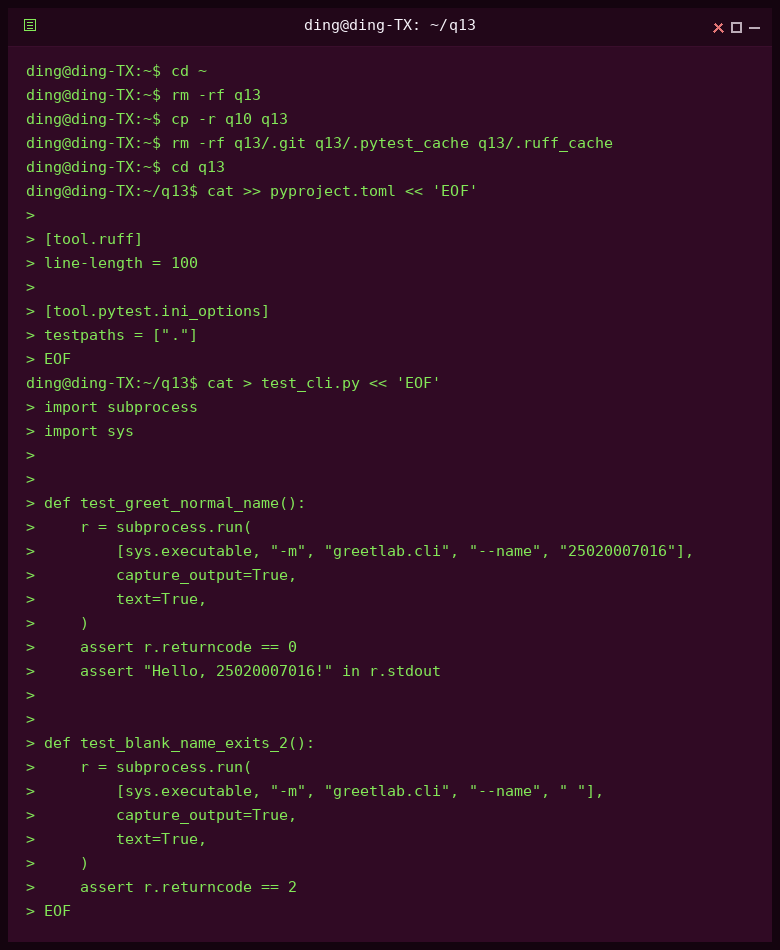
\includegraphics[width=0.85\textwidth]{q13_step1_setup.png}
\caption{第13题步骤1：pyproject 配置与两个测试}
\end{figure}

\textbf{步骤2：质量检查并修复。} 运行 \texttt{ruff check}，报告两个 \texttt{PLW1510} 错误：\texttt{subprocess.run} 未显式指定 \texttt{check} 参数。按提示为两处 \texttt{subprocess.run} 补充 \texttt{check=False}（测试中自行断言退出码，无需让子进程抛异常）；随后 \texttt{ruff format} 规范化代码，再次 \texttt{ruff check} 与 \texttt{ruff format --check} 全部通过。

\begin{figure}[H]
\centering
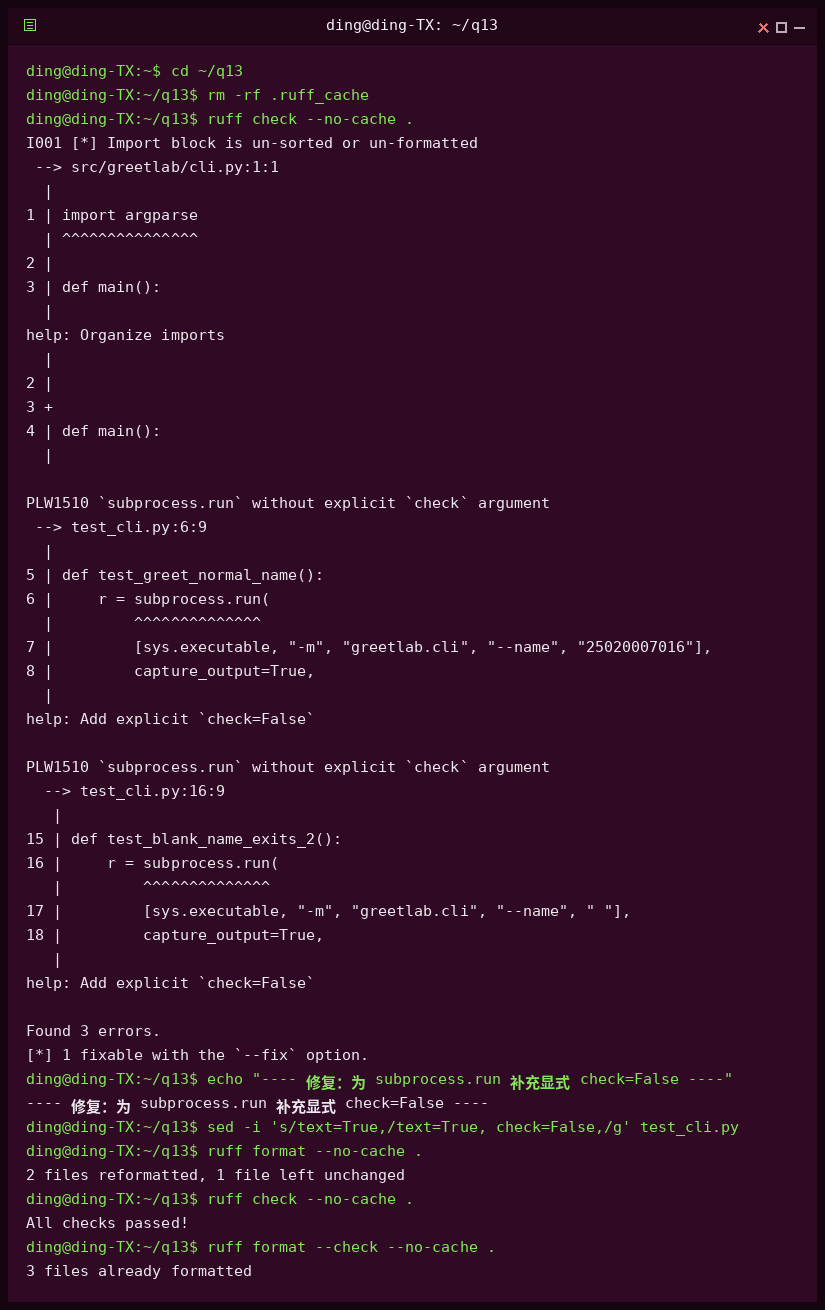
\includegraphics[width=0.85\textwidth]{q13_step2_quality_fix.png}
\caption{第13题步骤2：PLW1510 定位与修复}
\end{figure}

\textbf{步骤3：编写并运行 check.sh。} \texttt{check.sh} 用 \texttt{set -e} 保证任一步失败即整体退出，依次执行三步检查。运行输出三步全部通过，退出码 0。

\begin{figure}[H]
\centering
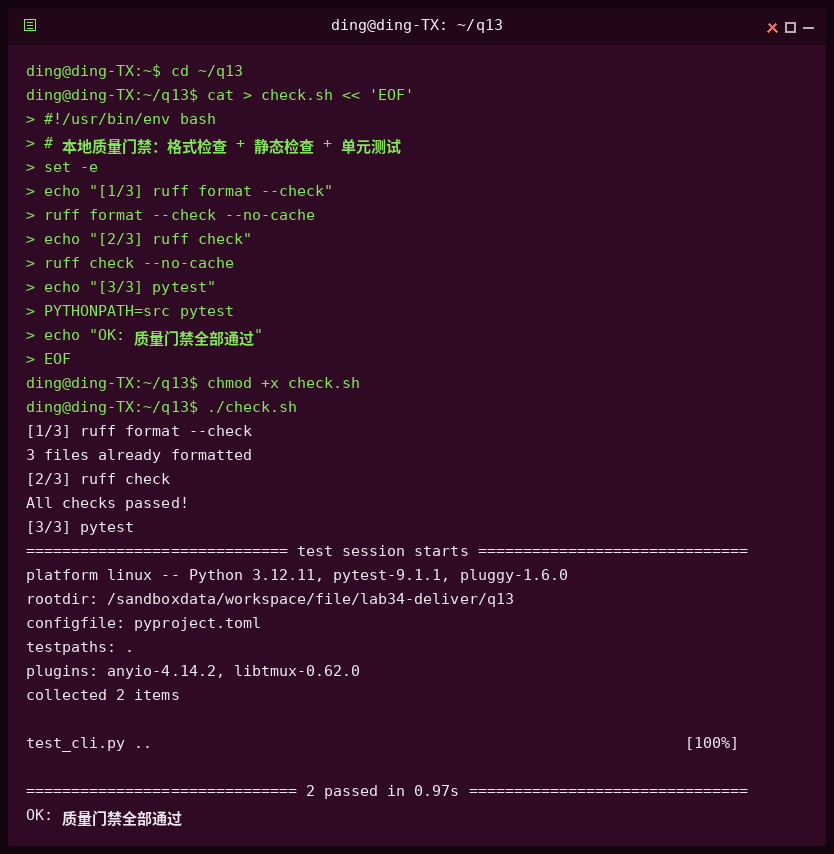
\includegraphics[width=0.85\textwidth]{q13_step3_check_sh.png}
\caption{第13题步骤3：check.sh 一键门禁通过}
\end{figure}

\subsubsection{关键技术点}

\begin{enumerate}
    \item \textbf{三层门禁}：格式检查（\texttt{format --check}）、静态检查（\texttt{ruff check}）、行为验证（\texttt{pytest}）各管一层，缺一不可。
    \item \textbf{PLW1510}：\texttt{subprocess.run} 不写 \texttt{check} 时默认忽略子进程失败，容易漏掉错误；显式 \texttt{check=False} 表明"故意不检查，由测试断言退出码"。
    \item \textbf{set -e 门禁语义}：脚本内任何命令非零退出都会终止脚本，保证门禁失败不会被后续命令掩盖。
    \item \textbf{不全局忽略规则}：问题靠修代码解决（补 \texttt{check=False}），而不是在配置里关闭该规则。
\end{enumerate}

% ------------------------------------------------------------
\subsection{第14题：Makefile 增量构建}

\subsubsection{题目要求}

在 \texttt{q14} 中编写 Makefile 管理数据统计与报告生成：

\begin{itemize}
    \item \texttt{make all} 依次执行 \texttt{stats.txt} 和 \texttt{report.txt} 两个目标。
    \item \texttt{make stats.txt} 运行 Python 脚本读取 \texttt{data.csv} 生成统计文件；\texttt{make report.txt} 依赖 \texttt{stats.txt}，运行脚本生成报告文件。
    \item \texttt{make clean} 只删除生成的文件；\texttt{all}、\texttt{clean} 声明为 \texttt{.PHONY}。
    \item 验证首次 make 生成两个产物；第二次无改动时不执行配方；\texttt{touch data.csv} 后再次 make，确认重新生成；clean 只删生成物。
\end{itemize}

\subsubsection{执行过程与结果}

\textbf{步骤1：创建数据与脚本。} 创建 \texttt{data.csv}（4 条姓名-成绩记录）、\texttt{stats.py}（读取 csv 计算总人数、最高分、最低分、平均分，写入 \texttt{stats.txt}）、\texttt{report.py}（读取 \texttt{stats.txt} 生成 \texttt{report.txt}）以及 Makefile。Makefile 中 \texttt{stats.txt} 依赖 \texttt{data.csv} 与 \texttt{stats.py}，\texttt{report.txt} 依赖 \texttt{stats.txt} 与 \texttt{report.py}。

\begin{figure}[H]
\centering
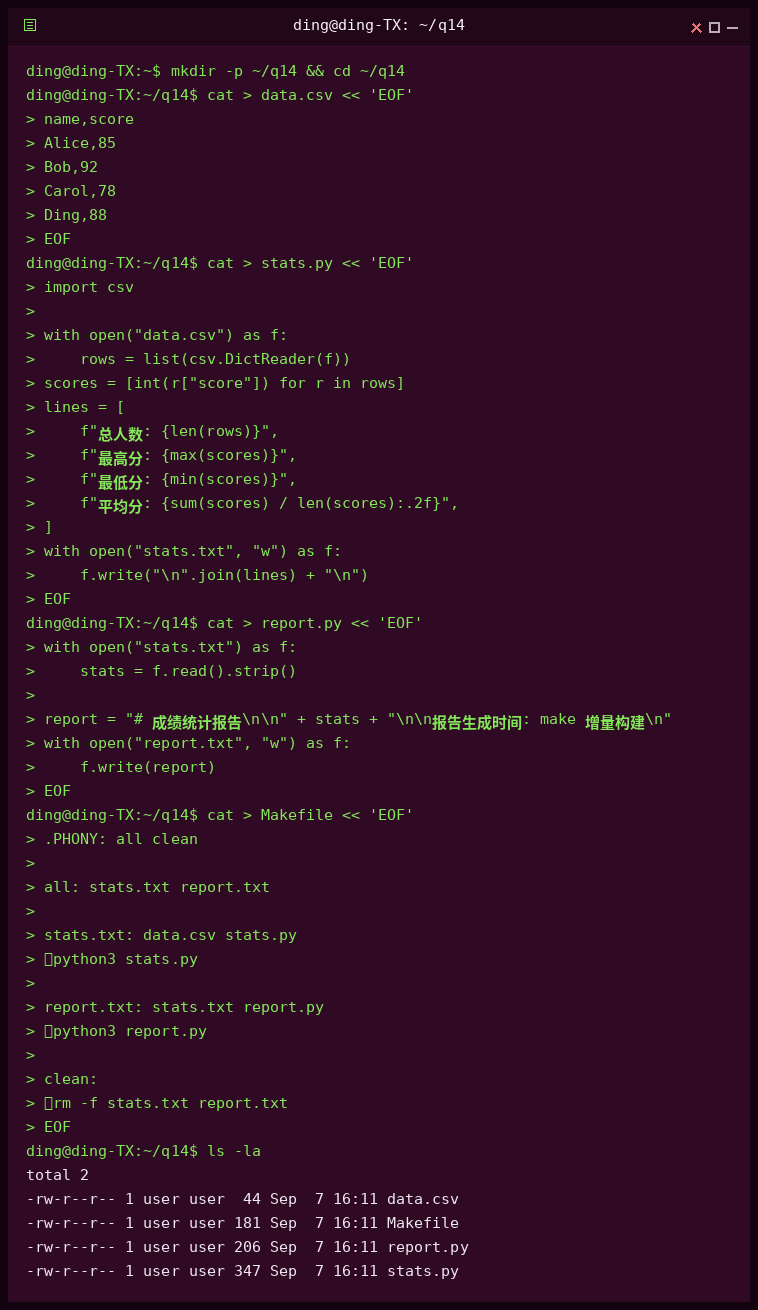
\includegraphics[width=0.8\textwidth]{q14_step1_files.png}
\caption{第14题步骤1：数据、脚本与 Makefile}
\end{figure}

\textbf{步骤2：首次构建与增量验证。} 首次 \texttt{make all} 依次执行 \texttt{stats.py} 和 \texttt{report.py}；再次执行 \texttt{make all}，输出 \texttt{Nothing to be done}，证明无改动时配方不会重复执行。

\begin{figure}[H]
\centering
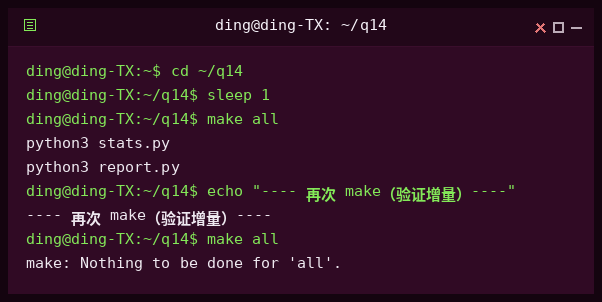
\includegraphics[width=0.8\textwidth]{q14_step2_make.png}
\caption{第14题步骤2：首次构建与二次无操作}
\end{figure}

\textbf{步骤3：依赖变更重建。} \texttt{touch data.csv} 后再次 \texttt{make all}，make 检测到数据文件更新，重新执行 \texttt{stats.py} 和 \texttt{report.py}；查看两个产物内容正确；最后 \texttt{make clean} 只删除 \texttt{stats.txt} 与 \texttt{report.txt}。

\begin{figure}[H]
\centering
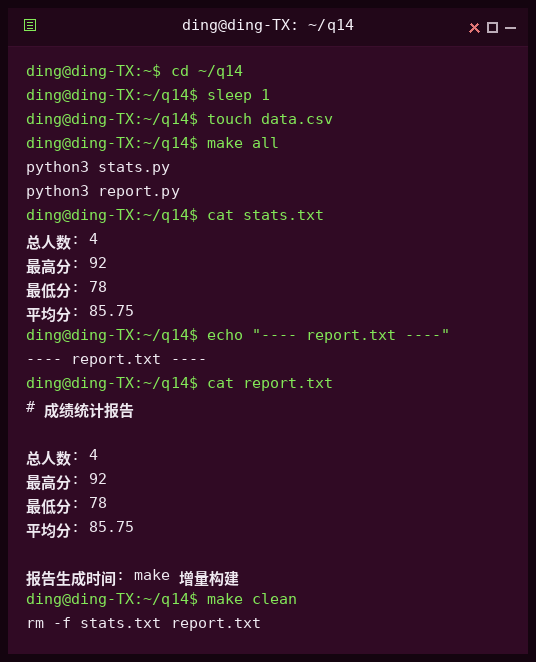
\includegraphics[width=0.8\textwidth]{q14_step3_rebuild.png}
\caption{第14题步骤3：touch 触发重建、产物与 clean}
\end{figure}

\subsubsection{关键技术点}

\begin{enumerate}
    \item \textbf{目标与依赖}：每个目标是文件，依赖是它重建所需的前置文件；make 比较目标与依赖的时间戳决定是否重建。
    \item \textbf{.PHONY}：\texttt{all}、\texttt{clean} 不是真实文件，声明为伪目标避免与同名文件冲突。
    \item \textbf{增量构建}：只重建依赖被改动的目标；\texttt{touch} 修改时间戳即可模拟数据更新，验证依赖链正确。
    \item \textbf{clean 语义}：只删生成物，不碰源文件（\texttt{data.csv}、脚本、Makefile 保留）。
\end{enumerate}

% ------------------------------------------------------------
\subsection{第15题：API 数据转报告}

\subsubsection{题目要求}

在 \texttt{q15} 中把本地 API 数据转换为可读报告：

\begin{itemize}
    \item 把给定 JSON 保存为 \texttt{packages.json}，并在 \texttt{q15} 目录运行 \texttt{python -m http.server 8000}。
    \item 使用 \texttt{curl -fsS} 获取 \texttt{http://127.0.0.1:8000/packages.json}。
    \item 使用 \texttt{jq} 筛选 \texttt{status} 为 \texttt{active} 且 \texttt{downloads} 不少于 100 的记录，并按 \texttt{downloads} 降序、\texttt{name} 升序排列。
    \item 编写 \texttt{api\_report.sh}，把结果生成 \texttt{summary.md}，包含标题和 \texttt{name/version/downloads} 三列表格。
\end{itemize}

\subsubsection{执行过程与结果}

\textbf{步骤1：启动本地服务。} 创建 \texttt{packages.json}（5 条软件包记录），后台启动 \texttt{python3 -m http.server 8000}，用 \texttt{curl -fsS} 获取 JSON，内容与给定数据一致。

\begin{figure}[H]
\centering
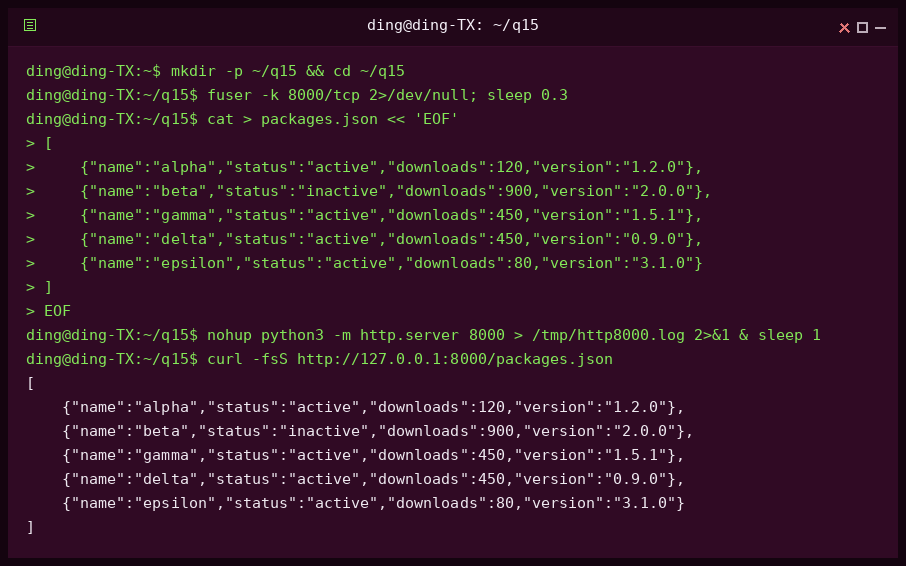
\includegraphics[width=0.85\textwidth]{q15_step1_server.png}
\caption{第15题步骤1：本地 HTTP 服务与 curl 获取}
\end{figure}

\textbf{步骤2：jq 筛选与排序。} 先筛选 \texttt{status == "active" and downloads >= 100}，得到 3 条记录（epsilon 因 downloads=80 被排除，beta 因 inactive 被排除）；再按 \texttt{downloads} 降序、\texttt{name} 升序排序，得到 delta、gamma、alpha。

\begin{figure}[H]
\centering
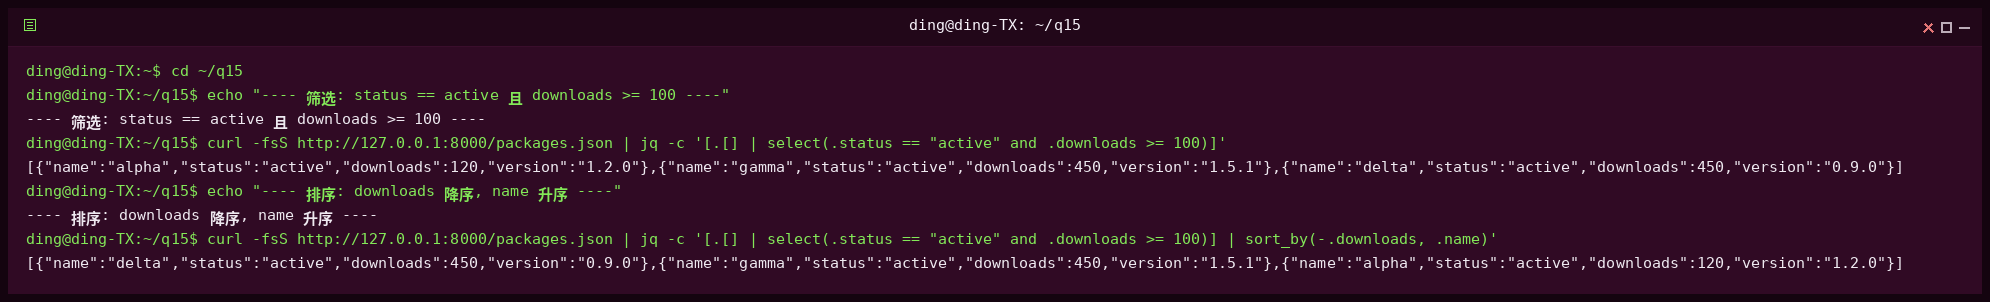
\includegraphics[width=0.85\textwidth]{q15_step2_jq.png}
\caption{第15题步骤2：jq 筛选与排序}
\end{figure}

\textbf{步骤3：脚本生成报告。} \texttt{api\_report.sh} 用管道把 curl 结果经 jq 转换为 Markdown 表格行，生成 \texttt{summary.md}，包含标题和三列表格。

\begin{figure}[H]
\centering
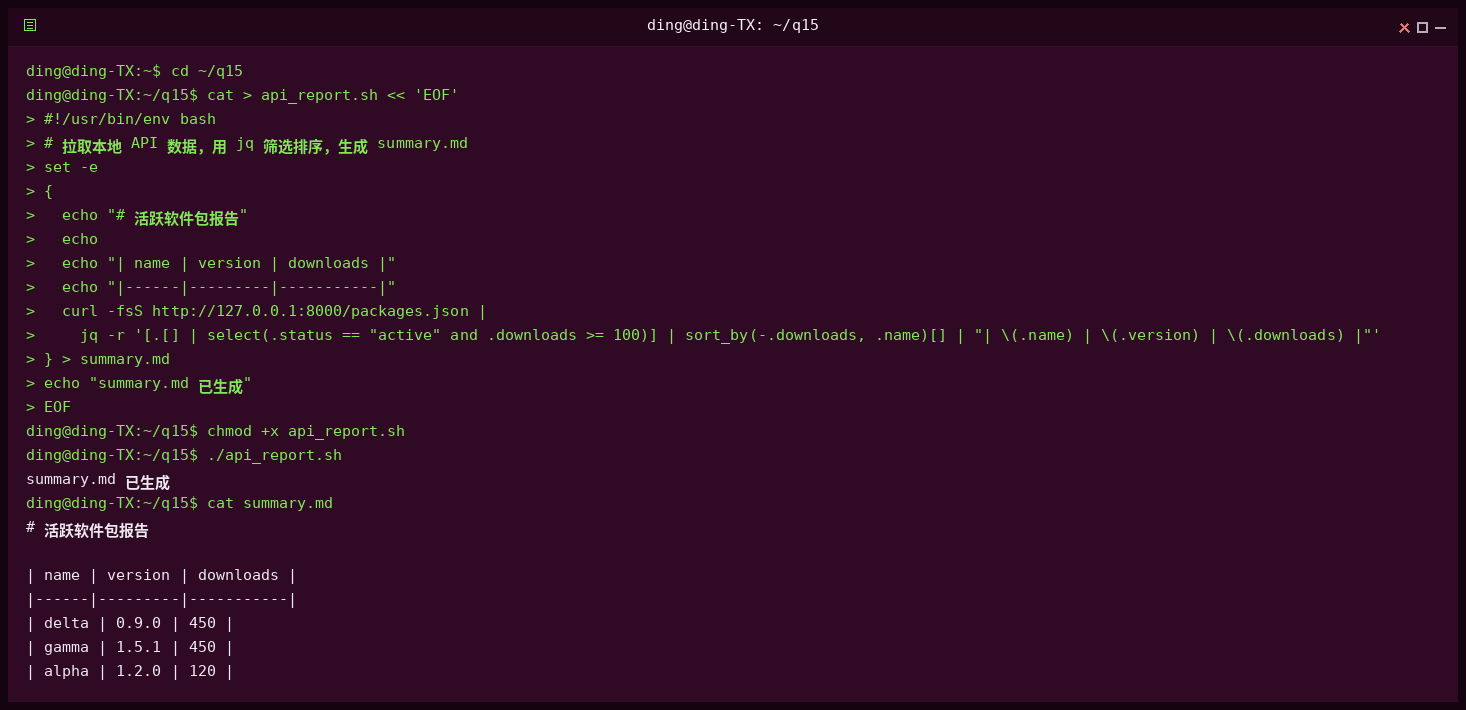
\includegraphics[width=0.85\textwidth]{q15_step3_report.png}
\caption{第15题步骤3：api\_report.sh 与生成的 summary.md}
\end{figure}

\subsubsection{关键技术点}

\begin{enumerate}
    \item \textbf{curl -fsS}：\texttt{-f} 在 HTTP 错误时失败退出，\texttt{-sS} 静默但保留错误信息，适合脚本中调用。
    \item \textbf{jq 管道筛选}：\texttt{select(.status == "active" and .downloads >= 100)} 完成过滤；\texttt{sort\_by(-.downloads, .name)} 先按下载量降序、再按名称升序。
    \item \textbf{CLI 约定}：把固定流程写进 \texttt{api\_report.sh}（\texttt{set -e}），重复执行结果一致，可纳入自动化。
\end{enumerate}

% ------------------------------------------------------------
\subsection{第16题：修复并交付一个陌生的小型工具仓库}

\subsubsection{题目要求}

复用第13题的项目，在 \texttt{q16} 中完成一次 15 分钟综合检查：

\begin{itemize}
    \item 复制 \texttt{q13} 为 \texttt{q16} 并初始化/继续使用 Git。
    \item 把问候语实现临时改成始终返回字面量 \texttt{Hello, name!}，运行 \texttt{check.sh} 确认测试失败；随后定位并修复。
    \item 编写最小 Makefile，包含 \texttt{check}、\texttt{build} 和 \texttt{clean}；\texttt{check} 调用 \texttt{check.sh}，\texttt{build} 生成 wheel。
    \item 运行 \texttt{make check} 和 \texttt{make build}，计算 wheel 的 SHA-256，并把最终改动提交为一个内容聚焦的 Git 提交。
\end{itemize}

\subsubsection{执行过程与结果}

\textbf{步骤1：基线提交与破坏。} 复制 \texttt{q13} 为 \texttt{q16}，创建 \texttt{.gitignore}（排除构建产物与缓存），\texttt{git init} 后提交基线；把 \texttt{print(f"Hello, \{a.name\}!")} 临时改为 \texttt{print("Hello, name!")}，运行 \texttt{check.sh}，正常姓名测试失败（输出不符合断言）。

\begin{figure}[H]
\centering
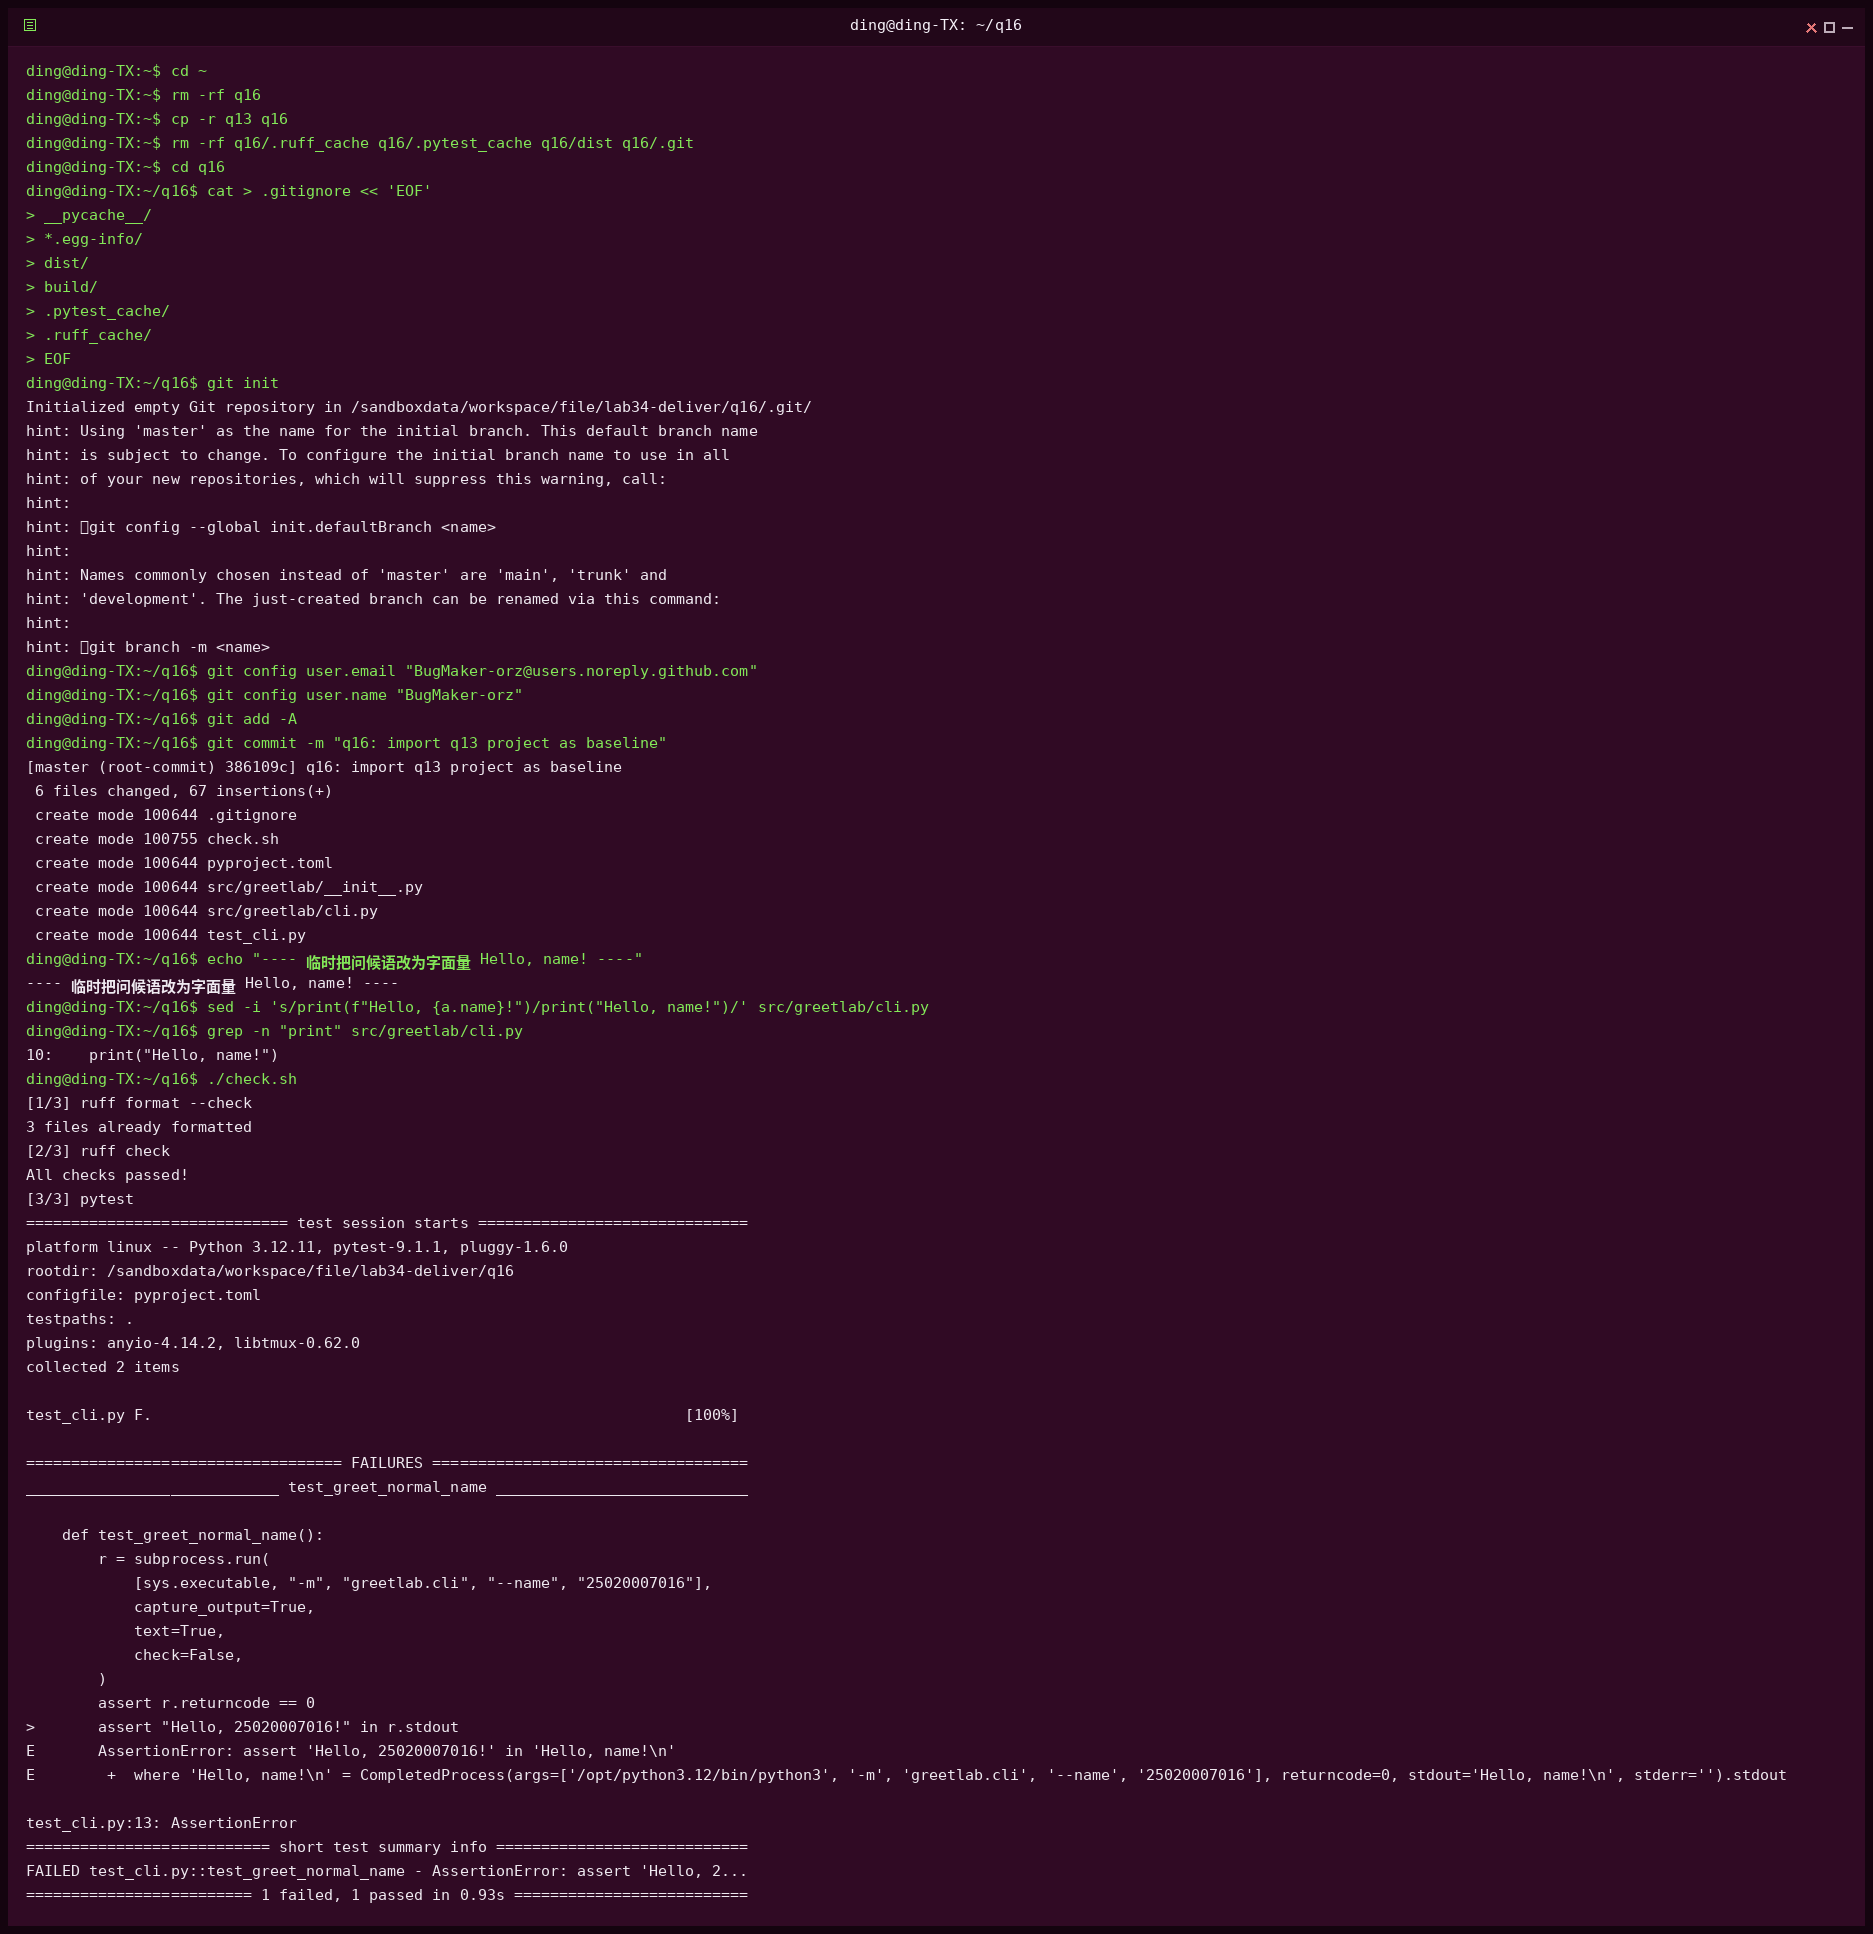
\includegraphics[width=0.85\textwidth]{q16_step1_break.png}
\caption{第16题步骤1：临时破坏后门禁失败}
\end{figure}

\textbf{步骤2：定位并修复。} 把实现改回 \texttt{f-string}，编写最小 Makefile（\texttt{check} 调用 \texttt{./check.sh}，\texttt{build} 执行 \texttt{python3 -m build -q}，\texttt{clean} 删除 dist、build 与 egg-info），运行 \texttt{make check}，门禁全部通过。

\begin{figure}[H]
\centering
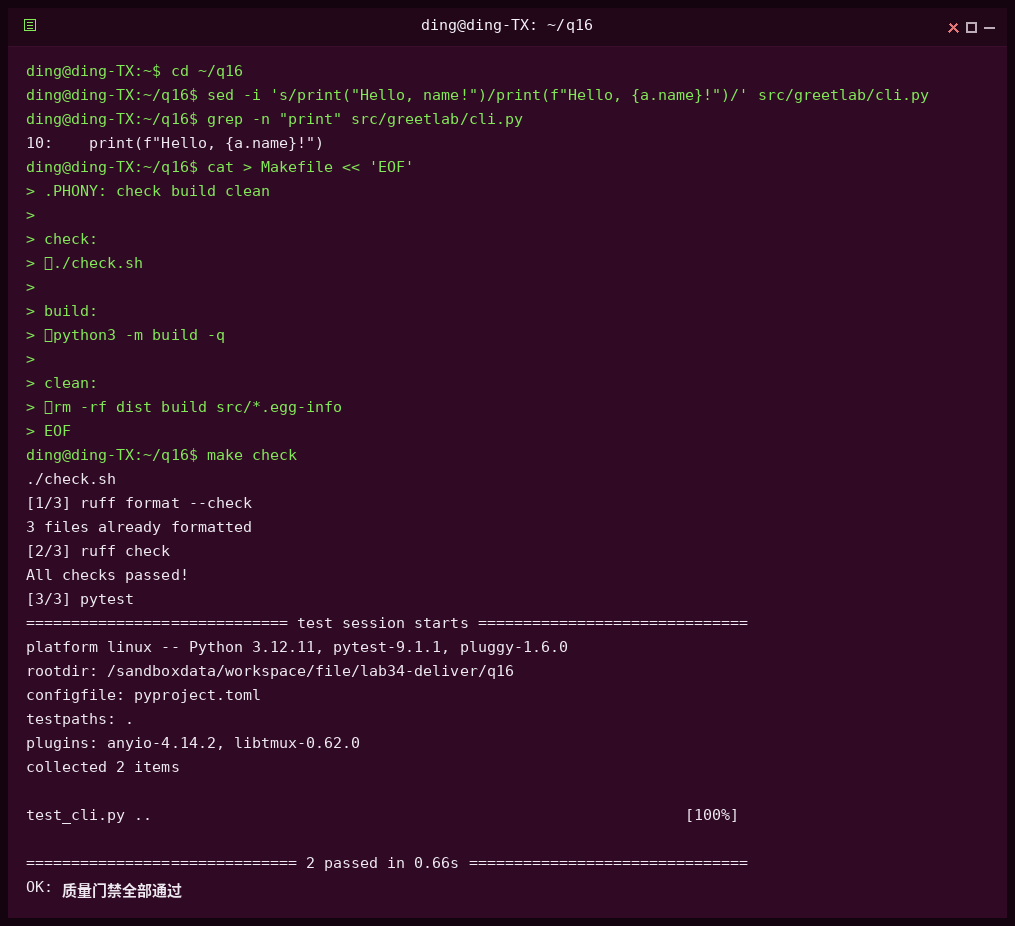
\includegraphics[width=0.85\textwidth]{q16_step2_fix.png}
\caption{第16题步骤2：修复后 make check 通过}
\end{figure}

\textbf{步骤3：构建与提交。} \texttt{make build} 生成 wheel 与 sdist，\texttt{sha256sum} 计算 wheel 的 SHA-256 校验值；最终改动（Makefile）提交为一个内容聚焦的提交，\texttt{git log} 显示两次提交：基线与修复。

\begin{figure}[H]
\centering
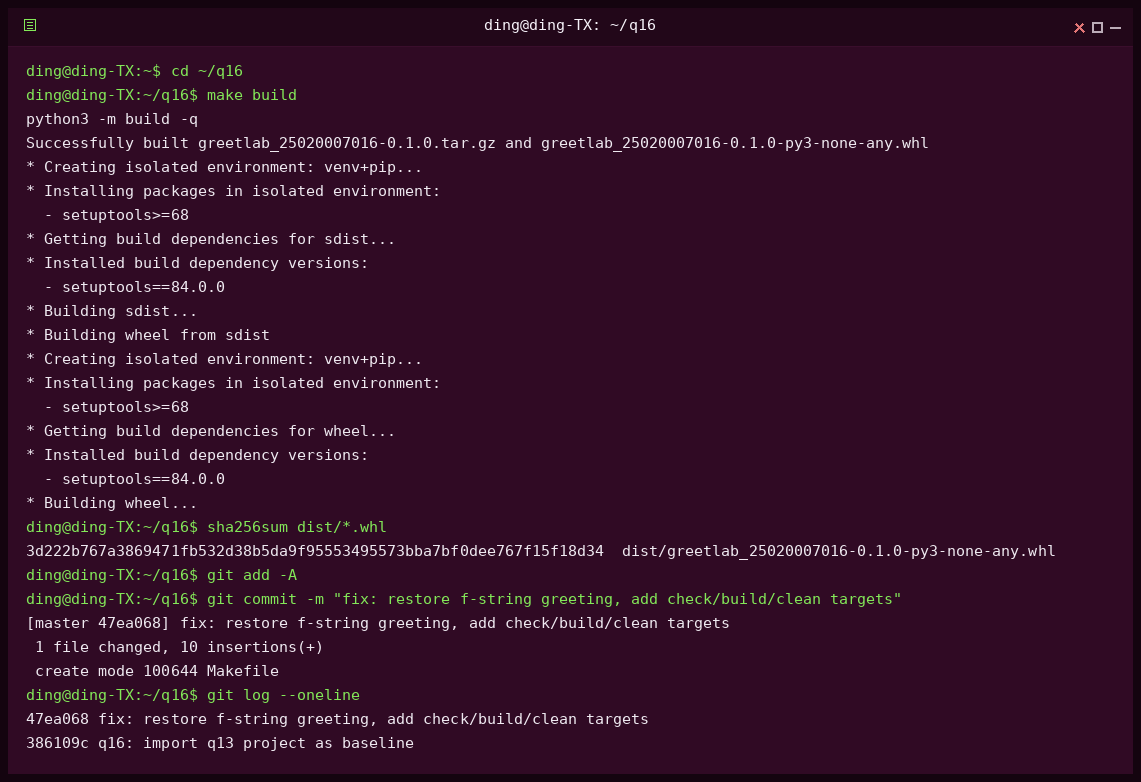
\includegraphics[width=0.85\textwidth]{q16_step3_build.png}
\caption{第16题步骤3：构建、SHA-256 与内容聚焦提交}
\end{figure}

\subsubsection{关键技术点}

\begin{enumerate}
    \item \textbf{先破坏再修复}：临时引入回归并让门禁失败，验证测试确实能抓住问题，修复后恢复通过，形成完整闭环。
    \item \textbf{Makefile 三目标}：\texttt{check} 复用已有门禁脚本，\texttt{build} 生成可分发包，\texttt{clean} 清理构建产物。
    \item \textbf{SHA-256 校验}：\texttt{sha256sum} 给出 wheel 的指纹，交付时可据此校验包完整性。
    \item \textbf{内容聚焦提交}：用 \texttt{.gitignore} 排除 dist、egg-info、缓存等构建产物，提交只包含有意义的源码与构建配置改动。
\end{enumerate}

% ============================================================
\section{进度说明}
% ============================================================

第四次实验共 4 题（第13、14、15、16题），已全部完成。第13题完成了 ruff + pytest 本地质量门禁；第14题完成了 Makefile 增量构建与 clean 验证；第15题完成了 HTTP 服务、curl/jq 数据处理与自动报告生成；第16题完成了陌生仓库的"破坏—失败—修复—构建—提交"综合检查。全部题目均配有终端截图与代码文件，本轮实验文件暂未推送 GitHub，整理后将按课程要求推送。

\vspace{1cm}
\noindent\rule{\textwidth}{0.4pt}
\begin{center}
\textit{报告结束}
\end{center}

\end{document}
